\chapter{Einleitung}			% Kapitelname

Die Zielsetzung des Projektes ist es einen Simulator für einen PIC16F84A Mikrocontroller zu schreiben. Dabei sollen verschieden Debug-Funktionen ebenfalls implementiert werden. Es soll Möglich sein ein korrekt geschriebenes Programm zu testen und zu debuggen.

\section{Was ist ein Simulator?}

Eine Simulation ist ein möglichst realitätsnahes Nachbilden von Geschehen der Wirklichkeit. Aus Sicherheits- und Kostengründen ist es für fast alle Anwendungsgebieten notwendig. Die gewonnenen Erkenntnisse können nach einer Simulation auf die Realität übertragen werden. Eine Simulation findet meistens nicht in Echtzeit statt (wie z.B. bei einer Emulation) sondern wird zu analytischen Zwecken langsamer als in der Realität nachgebildet.			% Einbinden der Unterkapitel
\section{Vor- und Nachteile eines Simulators}

\textbf{Vorteile:}
Durch eine Simulation k\"onnen Versuche die unter gef\"ahrlichen Umst\"anden stattfinden m\"ussen sicher nachgestellt werden (z.B. Crash-Simulationen mit Autos und Crash-Test-Dummys).
Aber auch Versuche die aus Kostengr\"unden in der Realit\"at oftmals schwierig nachzustellen sind k\"onnen durch Simulationen begrenzt ersetzt werden.
Durch den verlangsamten Ablauf einer Simulation sind au\ss erdem Fehler oder Ergebnisse leichter nachzuvollziehen als in der Wirklichkeit.
Im Falle des Mikrocontrollers k\"onnen Programme vor ihrem praktischen Einsatz getestet und debuggt werden um so m\"ogliche Fehler im Praxiseinsatz fr\"uhzeitig zu erkennen und auszubessern.\\
\\
\textbf{Nachteile:}
Eine Simulation ist meist durch begrenzte Ressourcen eingeschr\"ankt. Sei es die Rechenleistung einer Computersimulation oder Geld und Zeit die f\"ur eine Simulation eingesetzt werden m\"ussen. Oftmals wird deswegen nur ein vereinfachtes Modell der Wirklichkeit eingesetzt. Durch diese Vereinfachung kann es zu ungenauen Messergebnisse oder Situationen kommen die in der Realit\"at vielleicht gar nicht vorkommen.
F\"ur den PIC16-Simulatior ist es wichtig m\"oglichst fehlerfrei und genau zu arbeiten da Fehler innerhalb der Simulation auf falsche R\"uckschl\"usse auf das f\"ur den Mikrocontroller entwickelte Programm f\"uhren k\"onnte. Auch zu bedenken ist es das die Laufzeit in der Simulation nicht der Realzeit entspricht und somit das Programm in der Realit\"at schneller sein w\"urde.			% Einbinden der Unterkapitel
\section{Mikrocontroller PIC16F84A}

Ein Mikrocontroller ist eine Art Mikrorechnersystem, bei welchem neben ROM und RAM auch Peripherieeinheiten wie Schnittstellen, Timer und Bussysteme auf einem einzigen Chip integriert sind.
Die Hauptanwendungsgebiete sind die Steuerungs-, Mess- und Regelungstechnik, sowie die Kommunikationstechnik und die Bildverarbeitung. Mikrocontroller sind in der Regel in Embedded Systems, in die Anwendung eingebettete Systeme, und somit in der Regel von au\ss en nicht sichtbar. Ebenso verf\"ugen sie, im Gegensatz zum PC, nicht \"uber eine direkte Bedien- und Prorgrammierschnittstelle zum Benutzer. Sie werden in der Regel einmal programmiert und installiert.

Der PIC16F84 Mikrocontroller ist ein 8 Bit Mikrocontroller mit RISC-Architektur (Reduced-Instruction-Set-Computing). Es wird also auf komplexe Befehle verzichtet und mit jedem Befehl kann auf jedes Register zugegriffen werden. Der Mikrocontroller besitzt durch die eingesetzte Harvard-Architektur bis zu 14 Bit gro\ss e Befehle w\"ahrend die Gr\"o\ss e des separaten Datenbusses nur 8 Bit betr\"agt.

\begin{figure}[htb]
\centering
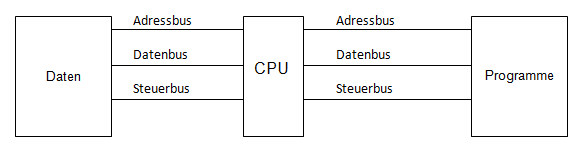
\includegraphics{Bilder/Harvard}
\caption{Harvard-Architektur}
\end{figure}

\newpage
Durch die Architektur ben\"otigen fast alle Anweisungen nur einen Instruction Cycle (Abarbeitung eines Maschinenbefehls).
Der PIC16 besitzt einen Stack mit Speicherplatz f\"ur 8 Adressen sowie 2 externe und 2 interne Interrupt Quellen. Dar\"uber hinaus besitzt der Pic16F ein gro\ss es Register, welches in zwei B\"anke unterteilt ist. Das Umschalten der B\"anke erfolgt im Programmcode. Die Speicherbereiche k\"onnen auch direkt \"uber ihre Registeradresse angesprochen werden.
			% Einbinden der Unterkapitel